本节介绍量子门，并展示其在 \MindQuantum\ 中的使用方式。我们将量子门分为三类：固定量子门、参数化量子门和自定义量子门。此外，我们使用 \code{on()} 方法设置目标量子比特和控制量子比特，并使用 \code{controlled()} 函数为多个量子门添加控制量子比特。

\subsubsection{量子门概述}

在量子计算中，量子门是操控量子比特的基本操作，而量子比特是量子信息的基本单位。类似于作用在比特上的经典逻辑门，量子门作用在量子比特上，并在数学上由酉矩阵表示，从而保持量子态的归一性和可逆性。

量子门通过执行旋转、翻转和生成纠缠等操作，成为构造量子线路和实现量子算法的核心。这些操作赋予量子计算机区别于经典计算机的独特计算能力。

量子门可以根据其作用的量子比特数量进行分类：单量子比特门修改单个量子比特的状态，多量子比特门则促成量子比特之间的相互作用，从而实现复杂量子操作和纠缠。量子门也可以分为非参数化门（例如 \X、\Y、\Z、\H）和参数化门（例如 \RX、\RY、\RZ），后者提供了额外的计算灵活性。在 \MindQuantum\ 中，这些量子门都可以便捷构造，其中也包括使用 \ParameterResolver\ 的参数化量子门。

\subsubsection{固定量子门}
固定量子门对量子态执行特定操作，并由酉矩阵表示。以下给出量子比特态 $\ket{\phi}=a\ket{0}+b\ket{1}$ 上的一些示例：

\begin{align*}
    I\ket{\phi} & =
    \begin{bmatrix}
        1 &  & 0 \\
        0 &  & 1
    \end{bmatrix}
    \begin{bmatrix}
        a \\
        b
    \end{bmatrix}=
    \begin{bmatrix}
        a \\
        b
    \end{bmatrix},  \\
    X\ket{\phi} & =
    \begin{bmatrix}
        0 &  & 1 \\
        1 &  & 0
    \end{bmatrix}
    \begin{bmatrix}
        a \\
        b
    \end{bmatrix}=
    \begin{bmatrix}
        b \\
        a
    \end{bmatrix},  \\
    Y\ket{\phi} & =
    \begin{bmatrix}
        0 & -i \\
        i & 0
    \end{bmatrix}
    \begin{bmatrix}
        a \\
        b
    \end{bmatrix}=
    \begin{bmatrix}
        -bi \\
        ai
    \end{bmatrix},  \\
    Z\ket{\phi} & =
    \begin{bmatrix}
        1 & 0 \\
        0 & -1
    \end{bmatrix}
    \begin{bmatrix}
        a \\
        b
    \end{bmatrix}=
    \begin{bmatrix}
        a \\
        -b
    \end{bmatrix}, \\
    H\ket{\phi} & =
    \frac{1}{\sqrt{2}}
    \begin{bmatrix}
        1 & 1  \\
        1 & -1
    \end{bmatrix}
    \begin{bmatrix}
        a \\
        b
    \end{bmatrix}=
    \frac{1}{\sqrt{2}}
    \begin{bmatrix}
        a+b \\
        a-b
    \end{bmatrix}.
\end{align*}

\MindQuantum\ 中的示例用法如下：
\begin{lstlisting}
from mindquantum.core.gates import H, SWAP

h = H.on(0)
swap = SWAP.on([0, 1])
print(swap)
\end{lstlisting}
输出为：
\begin{lstlisting}
SWAP(0 1)
\end{lstlisting}

\subsubsection{参数化量子门}
Pauli 矩阵是一类非常重要的矩阵，它们构成了算符空间的一组基。当 Pauli 矩阵出现在指数中时，可以得到三类有用的酉算符，即分别对应 $\hat{x}, \hat{y}, \hat{z}$ 方向的旋转算符，定义如下：

\begin{align*}
    Rx(\theta) & =
    e^{-\frac{i\theta X}{2}}=
    \cos{\frac{\theta}{2}}I-i\sin{\frac{\theta}{2}}X \\
               & =\begin{bmatrix}
        \cos{\frac{\theta}{2}}   &  & -i\sin{\frac{\theta}{2}} \\
        -i\sin{\frac{\theta}{2}} &  & \cos{\frac{\theta}{2}}
    \end{bmatrix},        \\
    Ry(\theta) & =
    e^{-\frac{i\theta Y}{2}}=
    \cos{\frac{\theta}{2}}I-i\sin{\frac{\theta}{2}}Y \\
               & =    \begin{bmatrix}
        \cos{\frac{\theta}{2}} &  & -\sin{\frac{\theta}{2}} \\
        \sin{\frac{\theta}{2}} &  & \cos{\frac{\theta}{2}}
    \end{bmatrix},    \\
    Rz(\theta) & =
    e^{-\frac{i\theta Z}{2}}=
    \cos{\frac{\theta}{2}}I-i\sin{\frac{\theta}{2}}Z \\
               & =    \begin{bmatrix}
        e^{\frac{-i\theta}{2}} &  & 0                     \\
        0                      &  & e^{\frac{i\theta}{2}}
    \end{bmatrix}.
\end{align*}


由于 $2\times2$ 矩阵的数量是无限的，量子门的数量也同样是无限的。根据 Z-Y 分解，任意单量子比特酉矩阵 $U$ 都可以表示为 $U=e^{i\alpha}Rz(\beta)Ry(\gamma)Rz(\delta)$。因此，为了构造通用量子门，需要使用参数来构造旋转门。由于 \ParameterResolver\ 支持三种初始化方式，\MindQuantum\ 也提供了三种初始化方法。以 RX 门为例：

\begin{lstlisting}
from mindquantum.core.gates import RX
from mindquantum.core.parameterresolver import ParameterResolver as PR
import numpy as np

rx1 = RX(0.5)
rx2 = RX('a')
rx3 = RX({'a': 0.2, 'b': 0.5})

a, b = PR('a'), PR('b')
rx4 = RX(0.2 * a + 0.5 * b)

mat_rx1 = rx1.matrix()
mat_rx4 = rx4.matrix(pr={'a': 1, 'b': 2})
\end{lstlisting}

请注意，在上述示例中，\code{rx1} 实际上是一个非参数化量子门，因为我们已经设置了旋转角 $\theta = 0.5$。

\subsubsection{自定义量子门}
在某些具体应用中，有时需要创建任意量子门。在 \MindQuantum\ 中，可以通过两种方法构造自定义量子门：

\textit{通用矩阵门} -- 如果已知某个量子门的矩阵表示，就可以在 \MindQuantum\ 中方便地构造该门。初始化 \UnivMathGate\ 需要两个参数，即量子门名称和矩阵值。如果矩阵不是酉矩阵，状态矢量将无法保持归一化。
示例：
\begin{lstlisting}
from mindquantum.core.gates import UnivMathGate
import numpy as np

x_mat = np.array([[0,1],[1,0]])
custom_X_gate = UnivMathGate('custom_X', x_mat).on(0, 1)
print(custom_X_gate)
\end{lstlisting}

输出：
\begin{lstlisting}
custom_X(0 <-: 1)
\end{lstlisting}

\textit{通用参数化门} -- 在某些应用中，我们需要构造参数会发生变化的参数化量子门。在 \MindQuantum\ 中，可以通过 \geneunivparameterizedgate\ 方便地构造自定义参数化量子门，其用法与 \RX\ 门基本一致。初始化这类量子门需要两个参数：其一是一个仅使用一个参数（类似 \RX\ 中的 theta）来生成酉矩阵的函数或方法，需要注意的是，即使生成的矩阵不是酉矩阵，也不会报错；其二是生成该矩阵导数的函数或方法，用于计算梯度。该方法支持生成任意量子比特算符，并可以通过 numba.JIT 加速性能。

示例：
\begin{lstlisting}
from mindquantum.core.gates import gene_univ_parameterized_gate

def matrix(theta):
    return np.array([[np.exp(1j * theta), 0],
                     [0, np.exp(-1j * theta)]])

def diff_matrix(theta):
    return 1j * np.array([[np.exp(1j * theta), 0],
                          [0, -np.exp(-1j * theta)]])

TestGate = gene_univ_parameterized_gate('Test', matrix, diff_matrix)

# 非参数化用法
test1 = TestGate(0.5).on(0)

# 参数化用法
test2 = TestGate('a').on(0)
\end{lstlisting}

\subsubsection{\texttt{on()} 方法}
对于某些受控量子门，我们需要指定量子门的目标量子比特和控制量子比特。在 \MindQuantum\ 中，可以通过 \code{on()} 方法实现该功能。此方法接收两个参数：一个是目标量子比特，另一个是控制量子比特；二者都可以是单个量子比特或多个量子比特。值得强调的是，任意量子门都可以添加任意控制操作。

示例：
\begin{lstlisting}
from mindquantum.core.gates import X

x = X.on(0, [1, 2])
print('Target qubit:{}, Control qubits:{}'.format(x.obj_qubits, x.ctrl_qubits))
\end{lstlisting}

输出：
\begin{lstlisting}
Target qubit:[0], Control qubits:[1, 2]
\end{lstlisting}

\subsubsection{\texttt{controlled()} 函数}
除 \code{on()} 方法外，我们还可以通过 \code{controlled()} 函数添加控制量子比特。\code{controlled()} 函数用于为任意量子线路或量子算符添加控制量子比特（可以有多个）。例如，我们构造一个仅包含两个量子比特的量子线路，并通过 \code{controlled()} 方法为其添加一个控制量子比特 q2：
\begin{lstlisting}
from mindquantum.algorithm.library import qft
from mindquantum.core.circuit import controlled

u1 = qft(range(2))
u2 = controlled(u1)
u2 = u2(2)
u2.svg()
\end{lstlisting}

如图~\ref{fig:controlled-method} 所示，此时 QFT 线路由 q2 控制。

\begin{figure}[h]
    \centering
    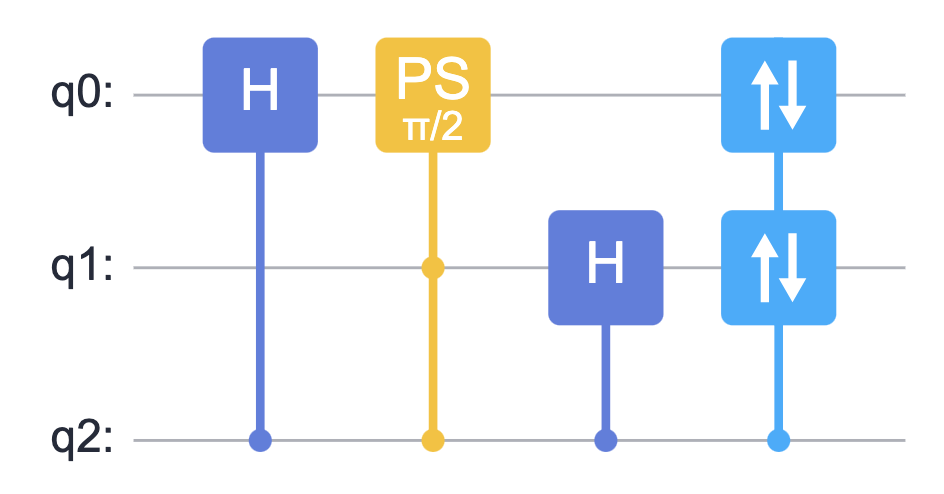
\includegraphics[width=0.9\linewidth]{2.3_figures/control.png}
    \caption{添加控制量子比特}
    \label{fig:controlled-method}
\end{figure}

此外，我们还可以批量为量子线路添加控制量子比特。在下面的示例中，目标量子比特分别为 q0 和 q1，对应的控制量子比特分别为 q2 和 q3：
\begin{lstlisting}
u = controlled(qft)
u = u([2, 3], [0, 1])
u.svg()
\end{lstlisting}

结果如图~\ref{fig:batch-control} 所示。
\begin{figure}[h]
    \centering
    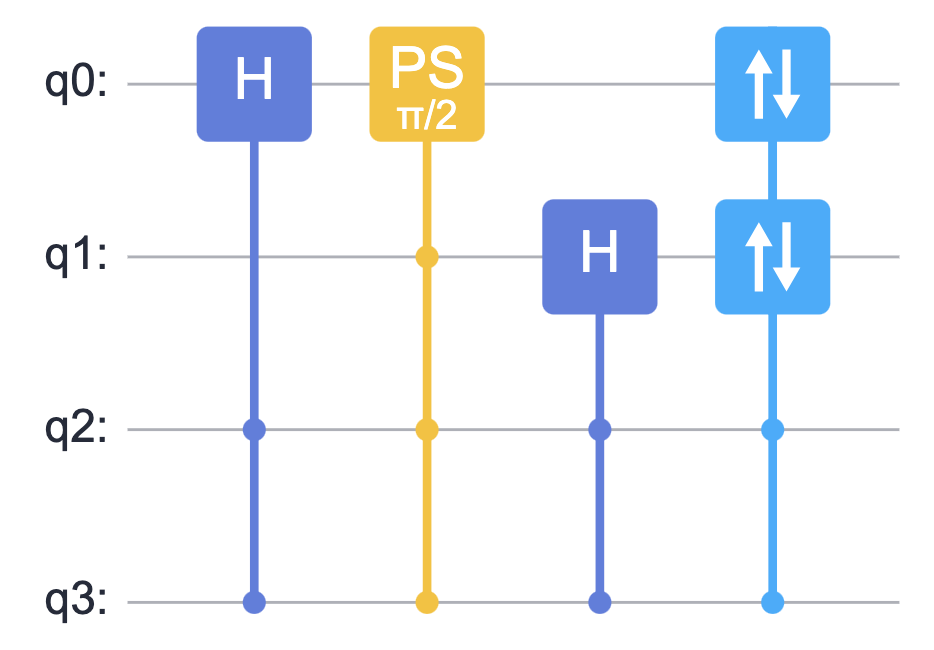
\includegraphics[width=0.9\linewidth]{2.3_figures/batch_control.png}
    \caption{批量添加控制量子比特}
    \label{fig:batch-control}
\end{figure}
